\chapter{Results \& Discussion}
%\textbf{Should include a reiteration of the experiments, and their outcome.  Together with a description (discussion).  Preamble should include a reminder of the aims and objectives together with a list of experiments to achieve these.  Should include many charts and other visualization with appropriate descriptions}.

\section{Data Collection Validation}

In the pre-processing experiment, the method used for collecting and filtering the 1000 Tweets.
To test that the distribution and collection was being done correctly, figures~\ref{fig:preprocessdist} and~\ref{fig:finaldist} where generated.


\begin{figure}[!htb]
\minipage{0.5\textwidth}
  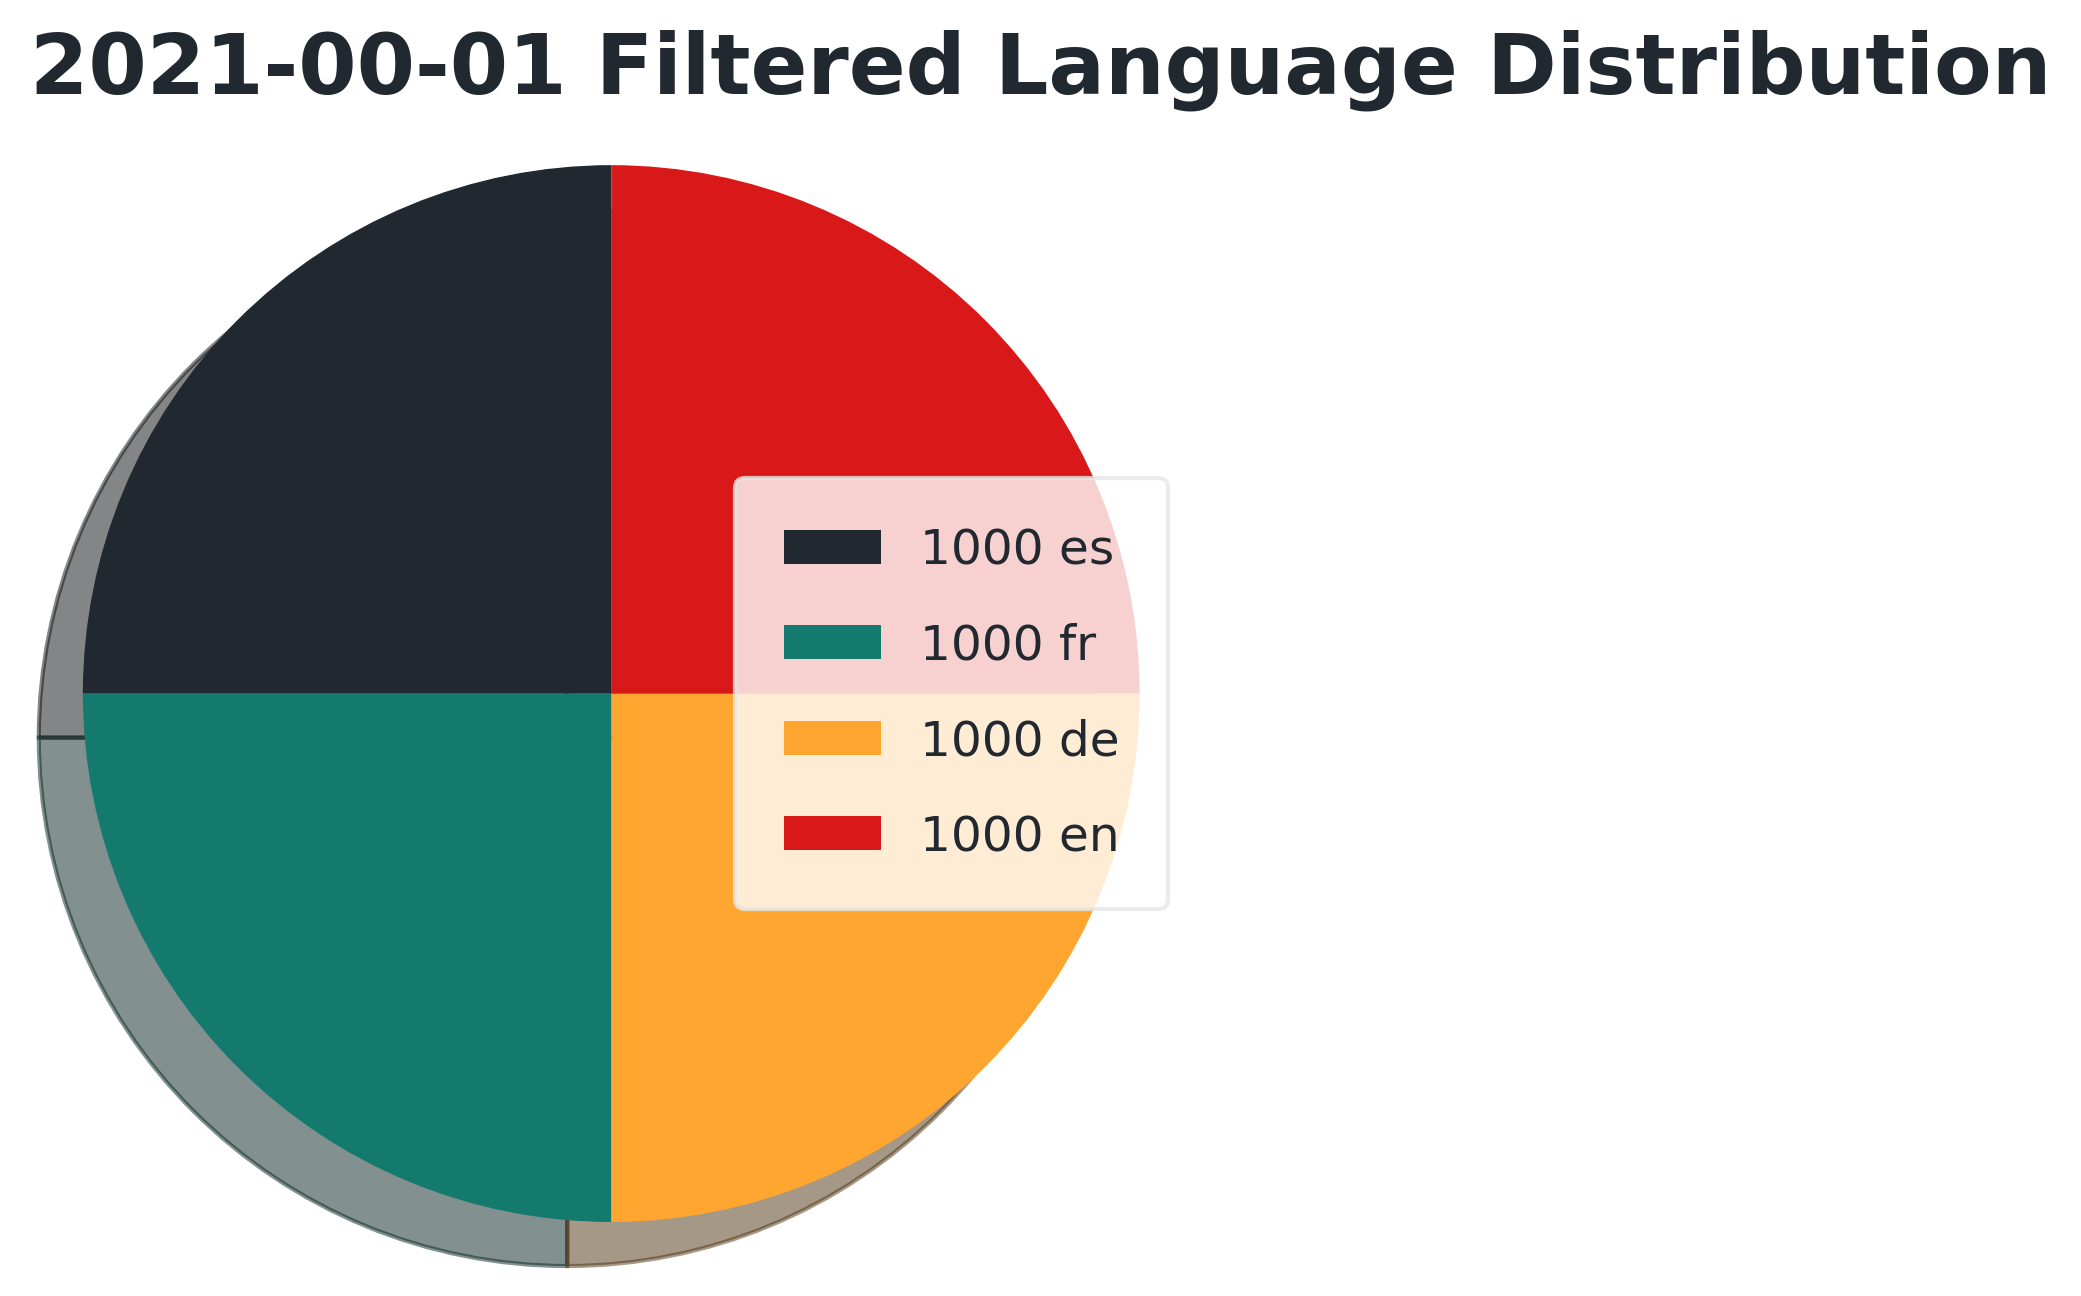
\includegraphics[width=\linewidth]{2021-00-01 Filtered Language Distribution.png}
  \caption{ }
  \label{fig:preprocessdist}
\endminipage\hfill
\minipage{0.5\textwidth}
  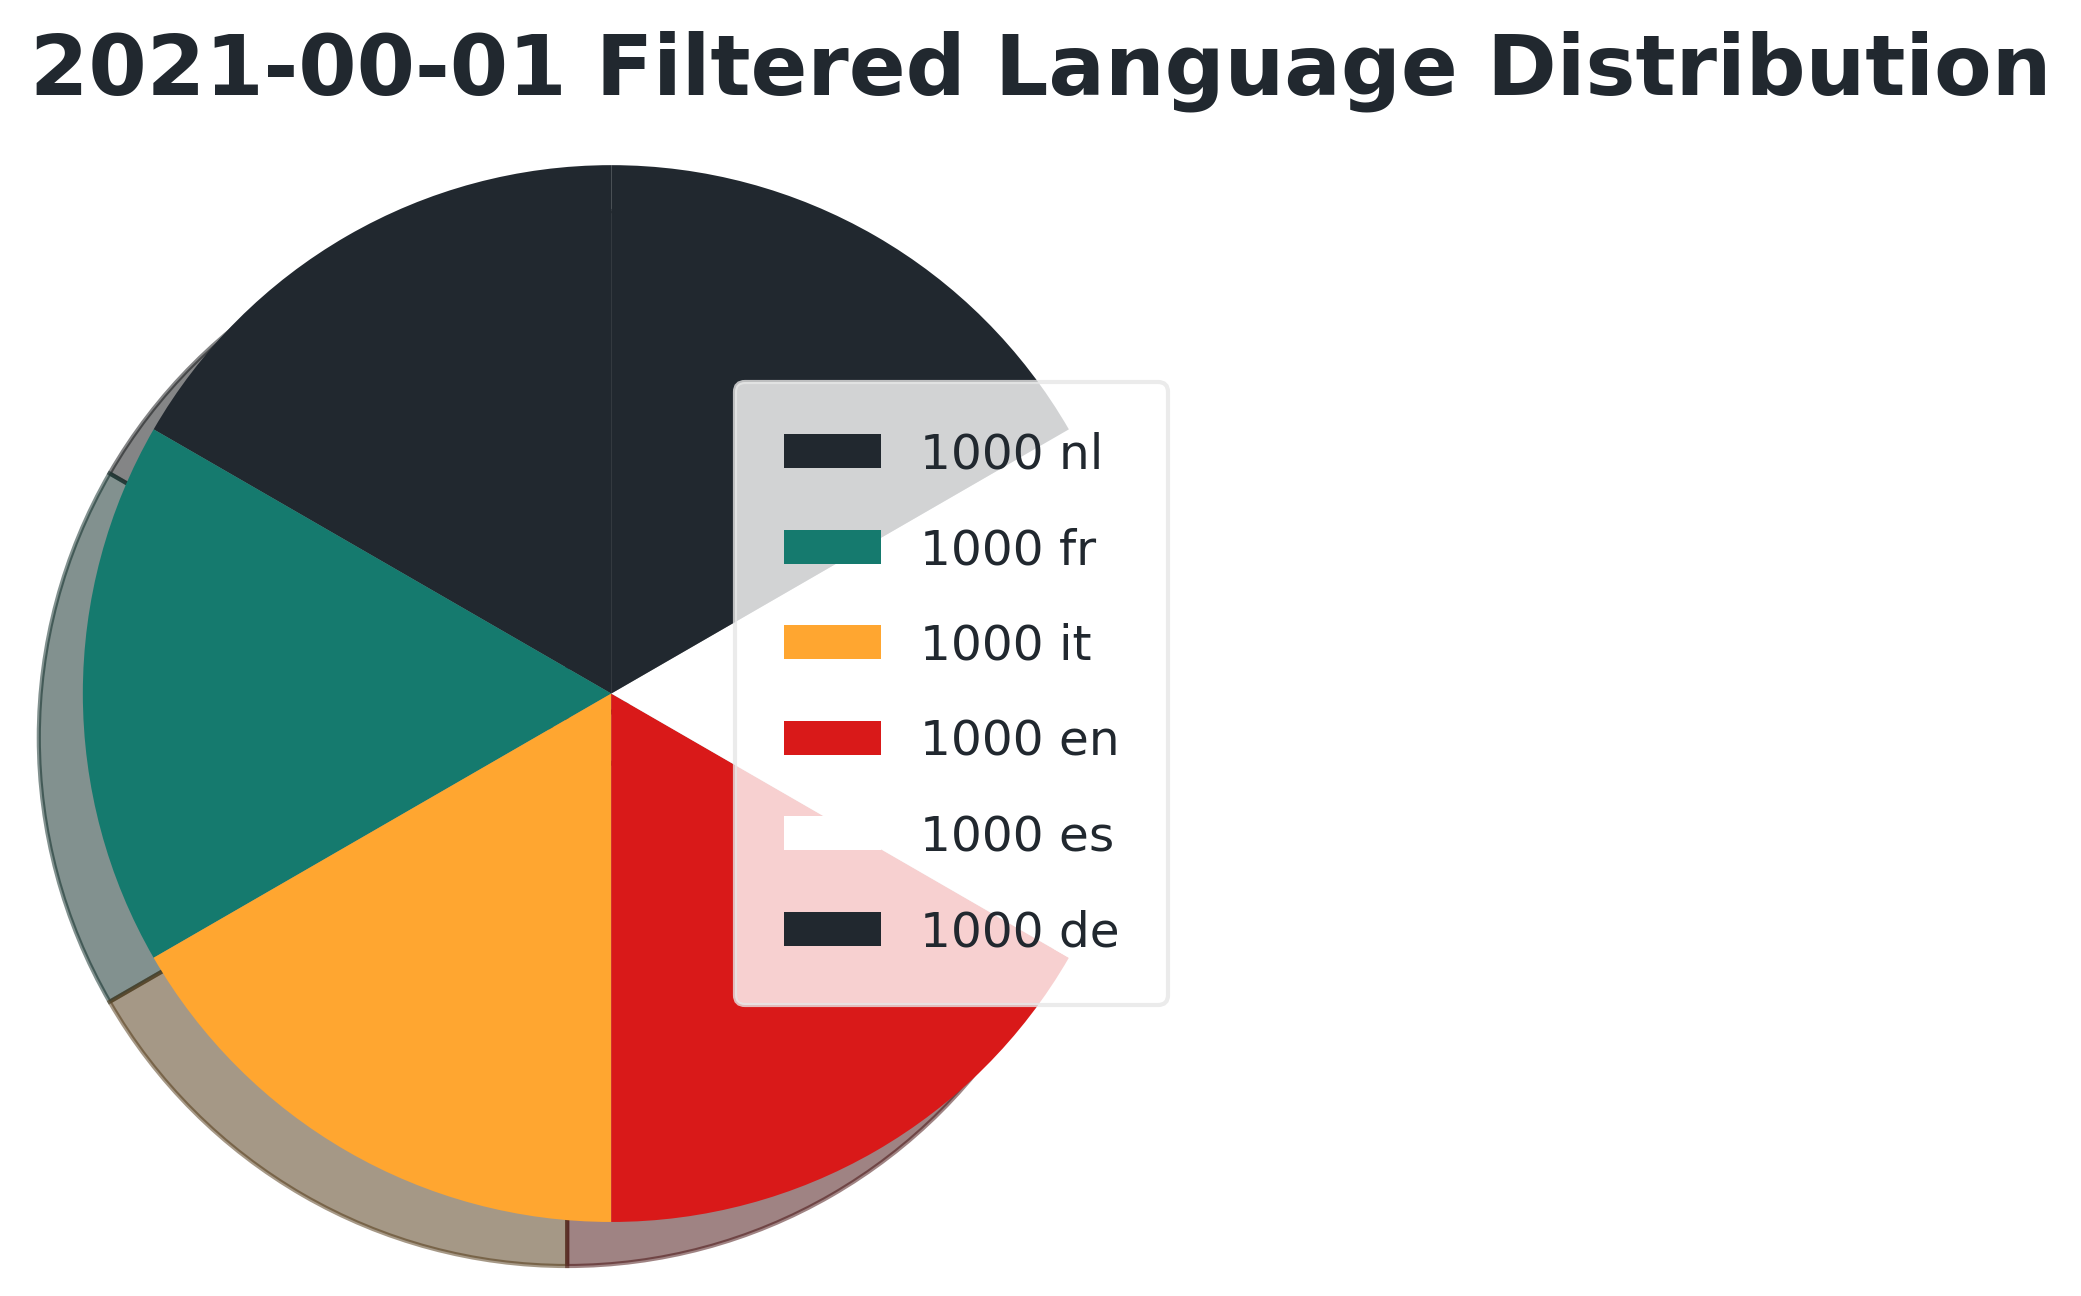
\includegraphics[width=\linewidth]{2021-01-01 Filtered Language Distribution - Final.png}
  \caption{ }
  \label{fig:finaldist}
\endminipage
\end{figure}


\section{Pre-Processing Effect}

The compound sentiment scores returned from the \ac{VADER} model was averaged and plotted for the 3 dates used in the experiment.
The 4 graphs produced, figures ~\ref{fig:EnglishPre},~\ref{fig:SpanishPre},~\ref{fig:FrenchPre} and~\ref{fig:GermanPre}, show a time series graph of each language over the 3 days which are 1 month apart.
The mean scores where also summed and the difference between the pre-processed and non-processed total was of 0.17\%.

\begin{figure}[!htb]
\minipage{0.5\textwidth}
  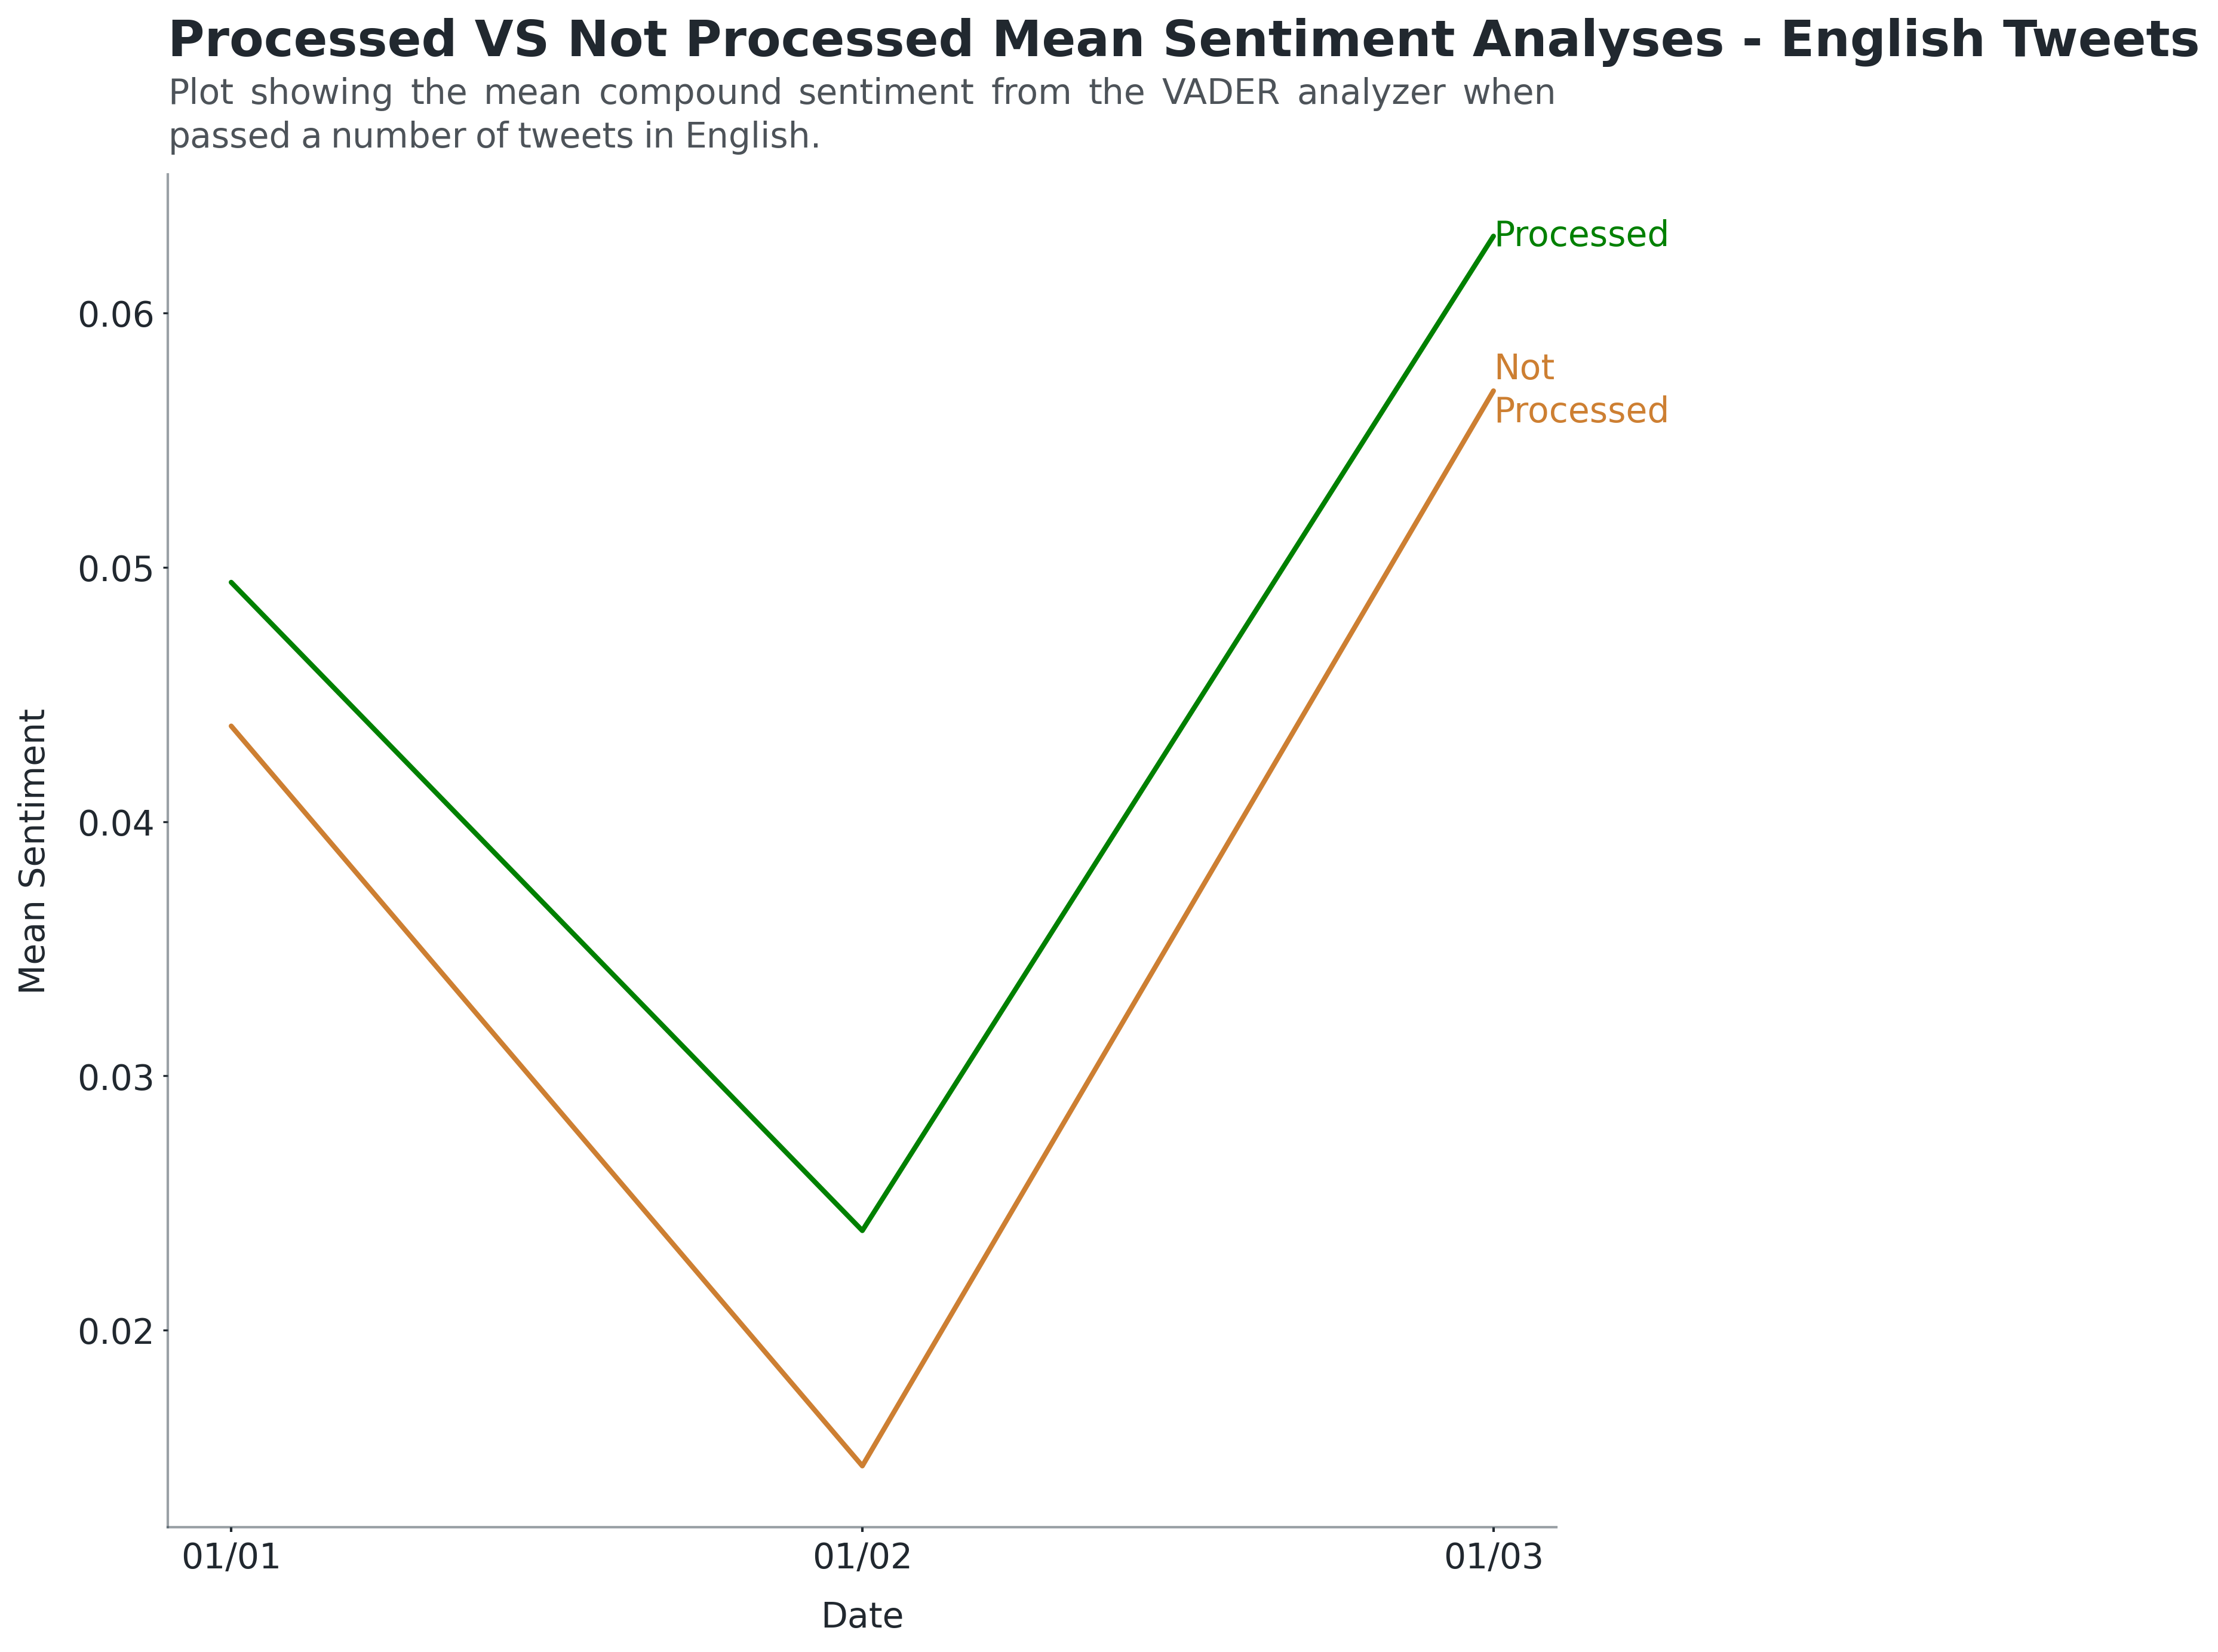
\includegraphics[width=\linewidth]{English Process VS NotProcessed.png}
  \caption{ }\label{fig:EnglishPre}
\endminipage\hfill
\minipage{0.5\textwidth}
  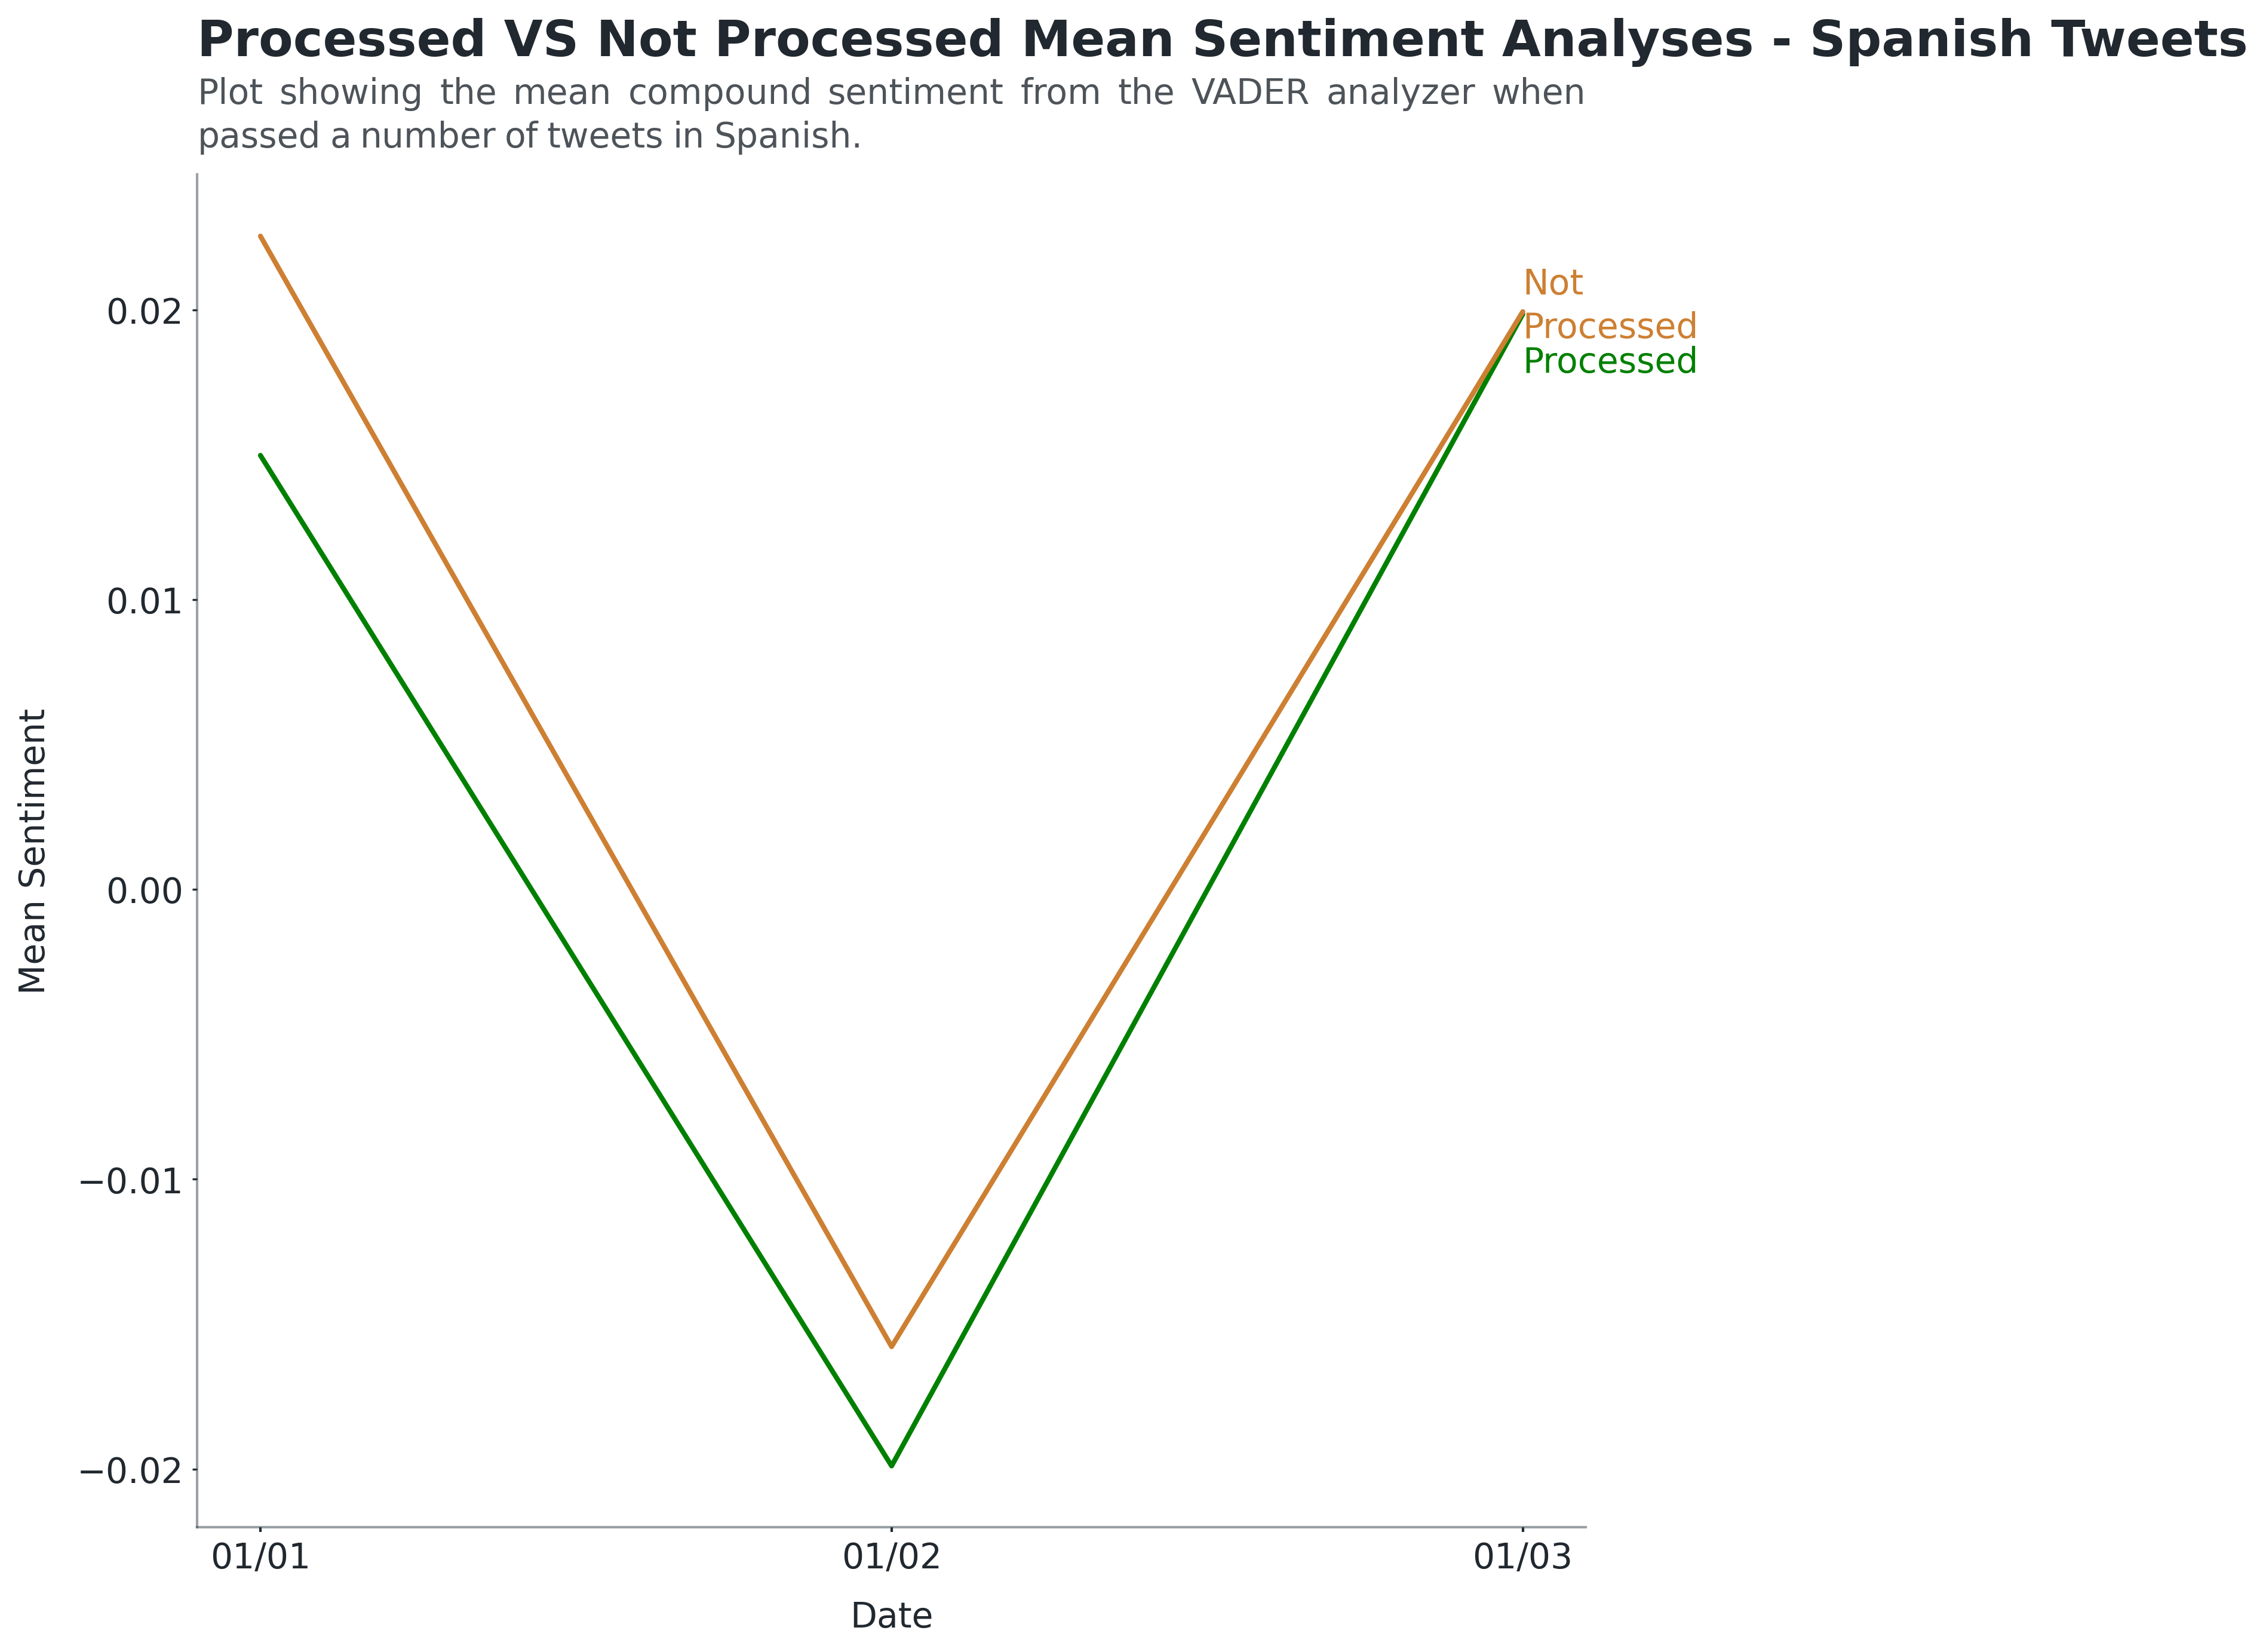
\includegraphics[width=\linewidth]{Spanish Process VS NotProcessed.png}
  \caption{ }\label{fig:SpanishPre}
\endminipage
\end{figure}
\begin{figure}[!htb]
\minipage{0.5\textwidth}
  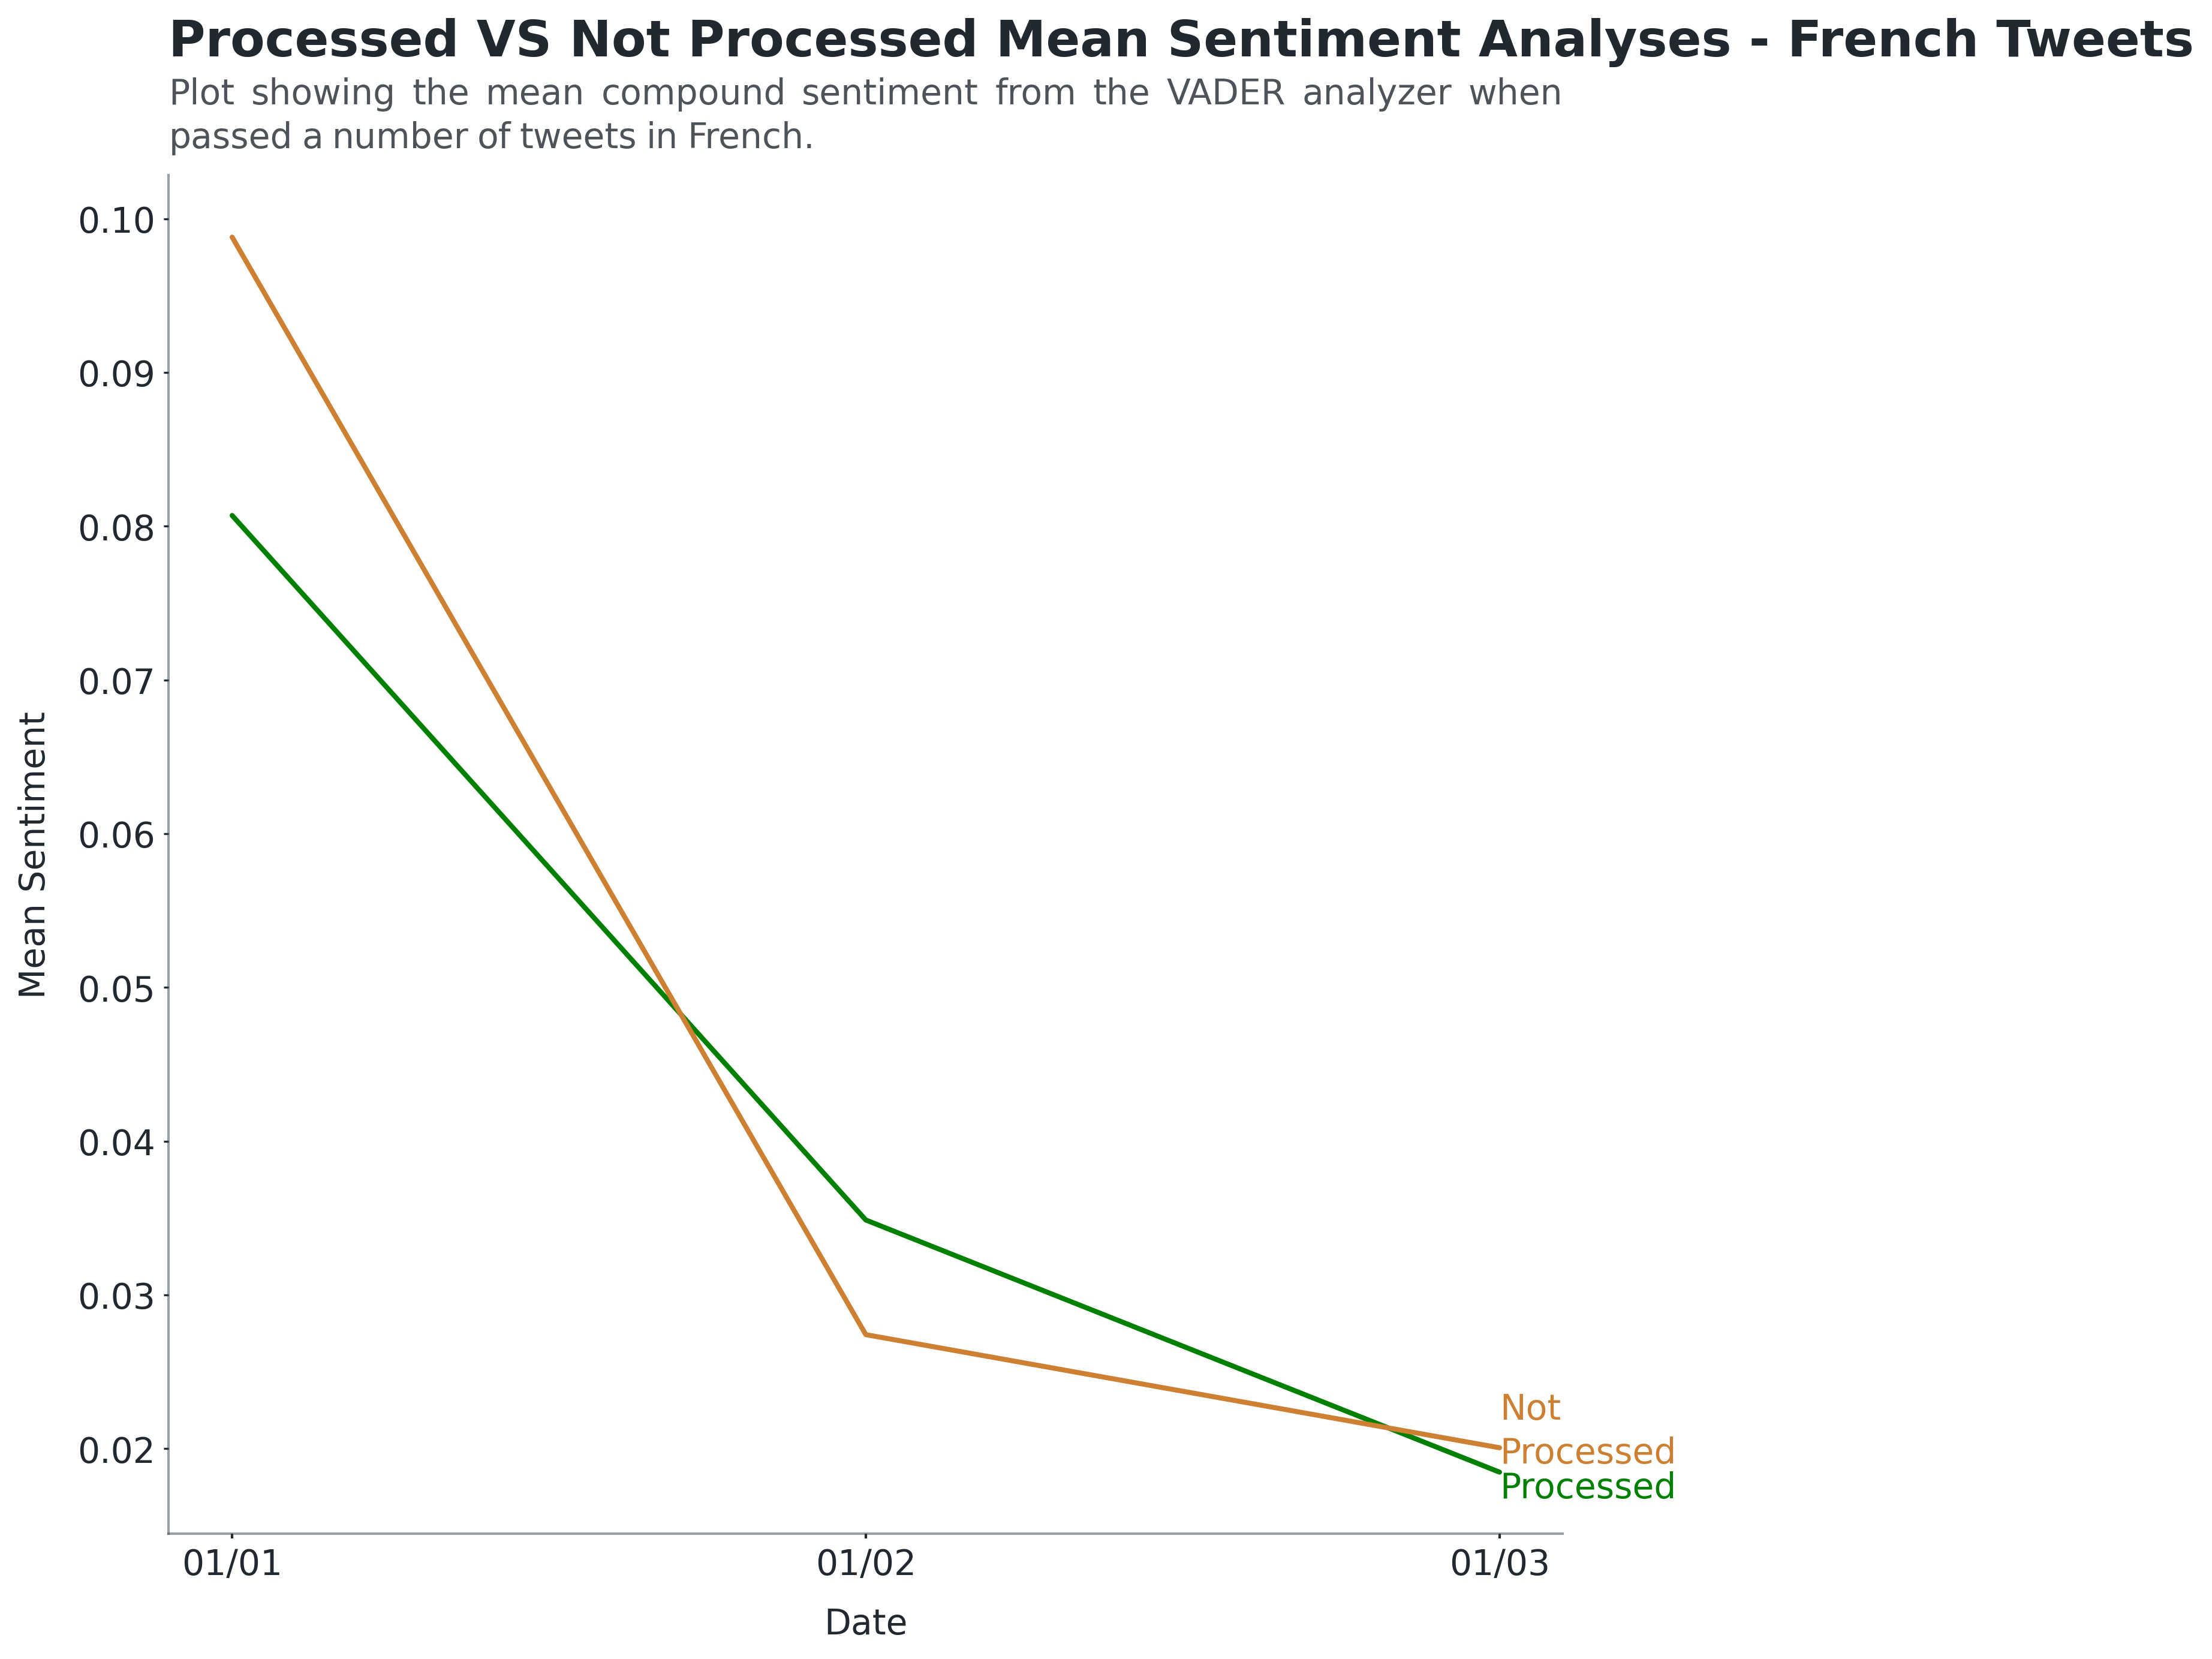
\includegraphics[width=\linewidth]{French Process VS NotProcessed.png}
  \caption{ }\label{fig:FrenchPre}
\endminipage\hfill
\minipage{0.5\textwidth}%
  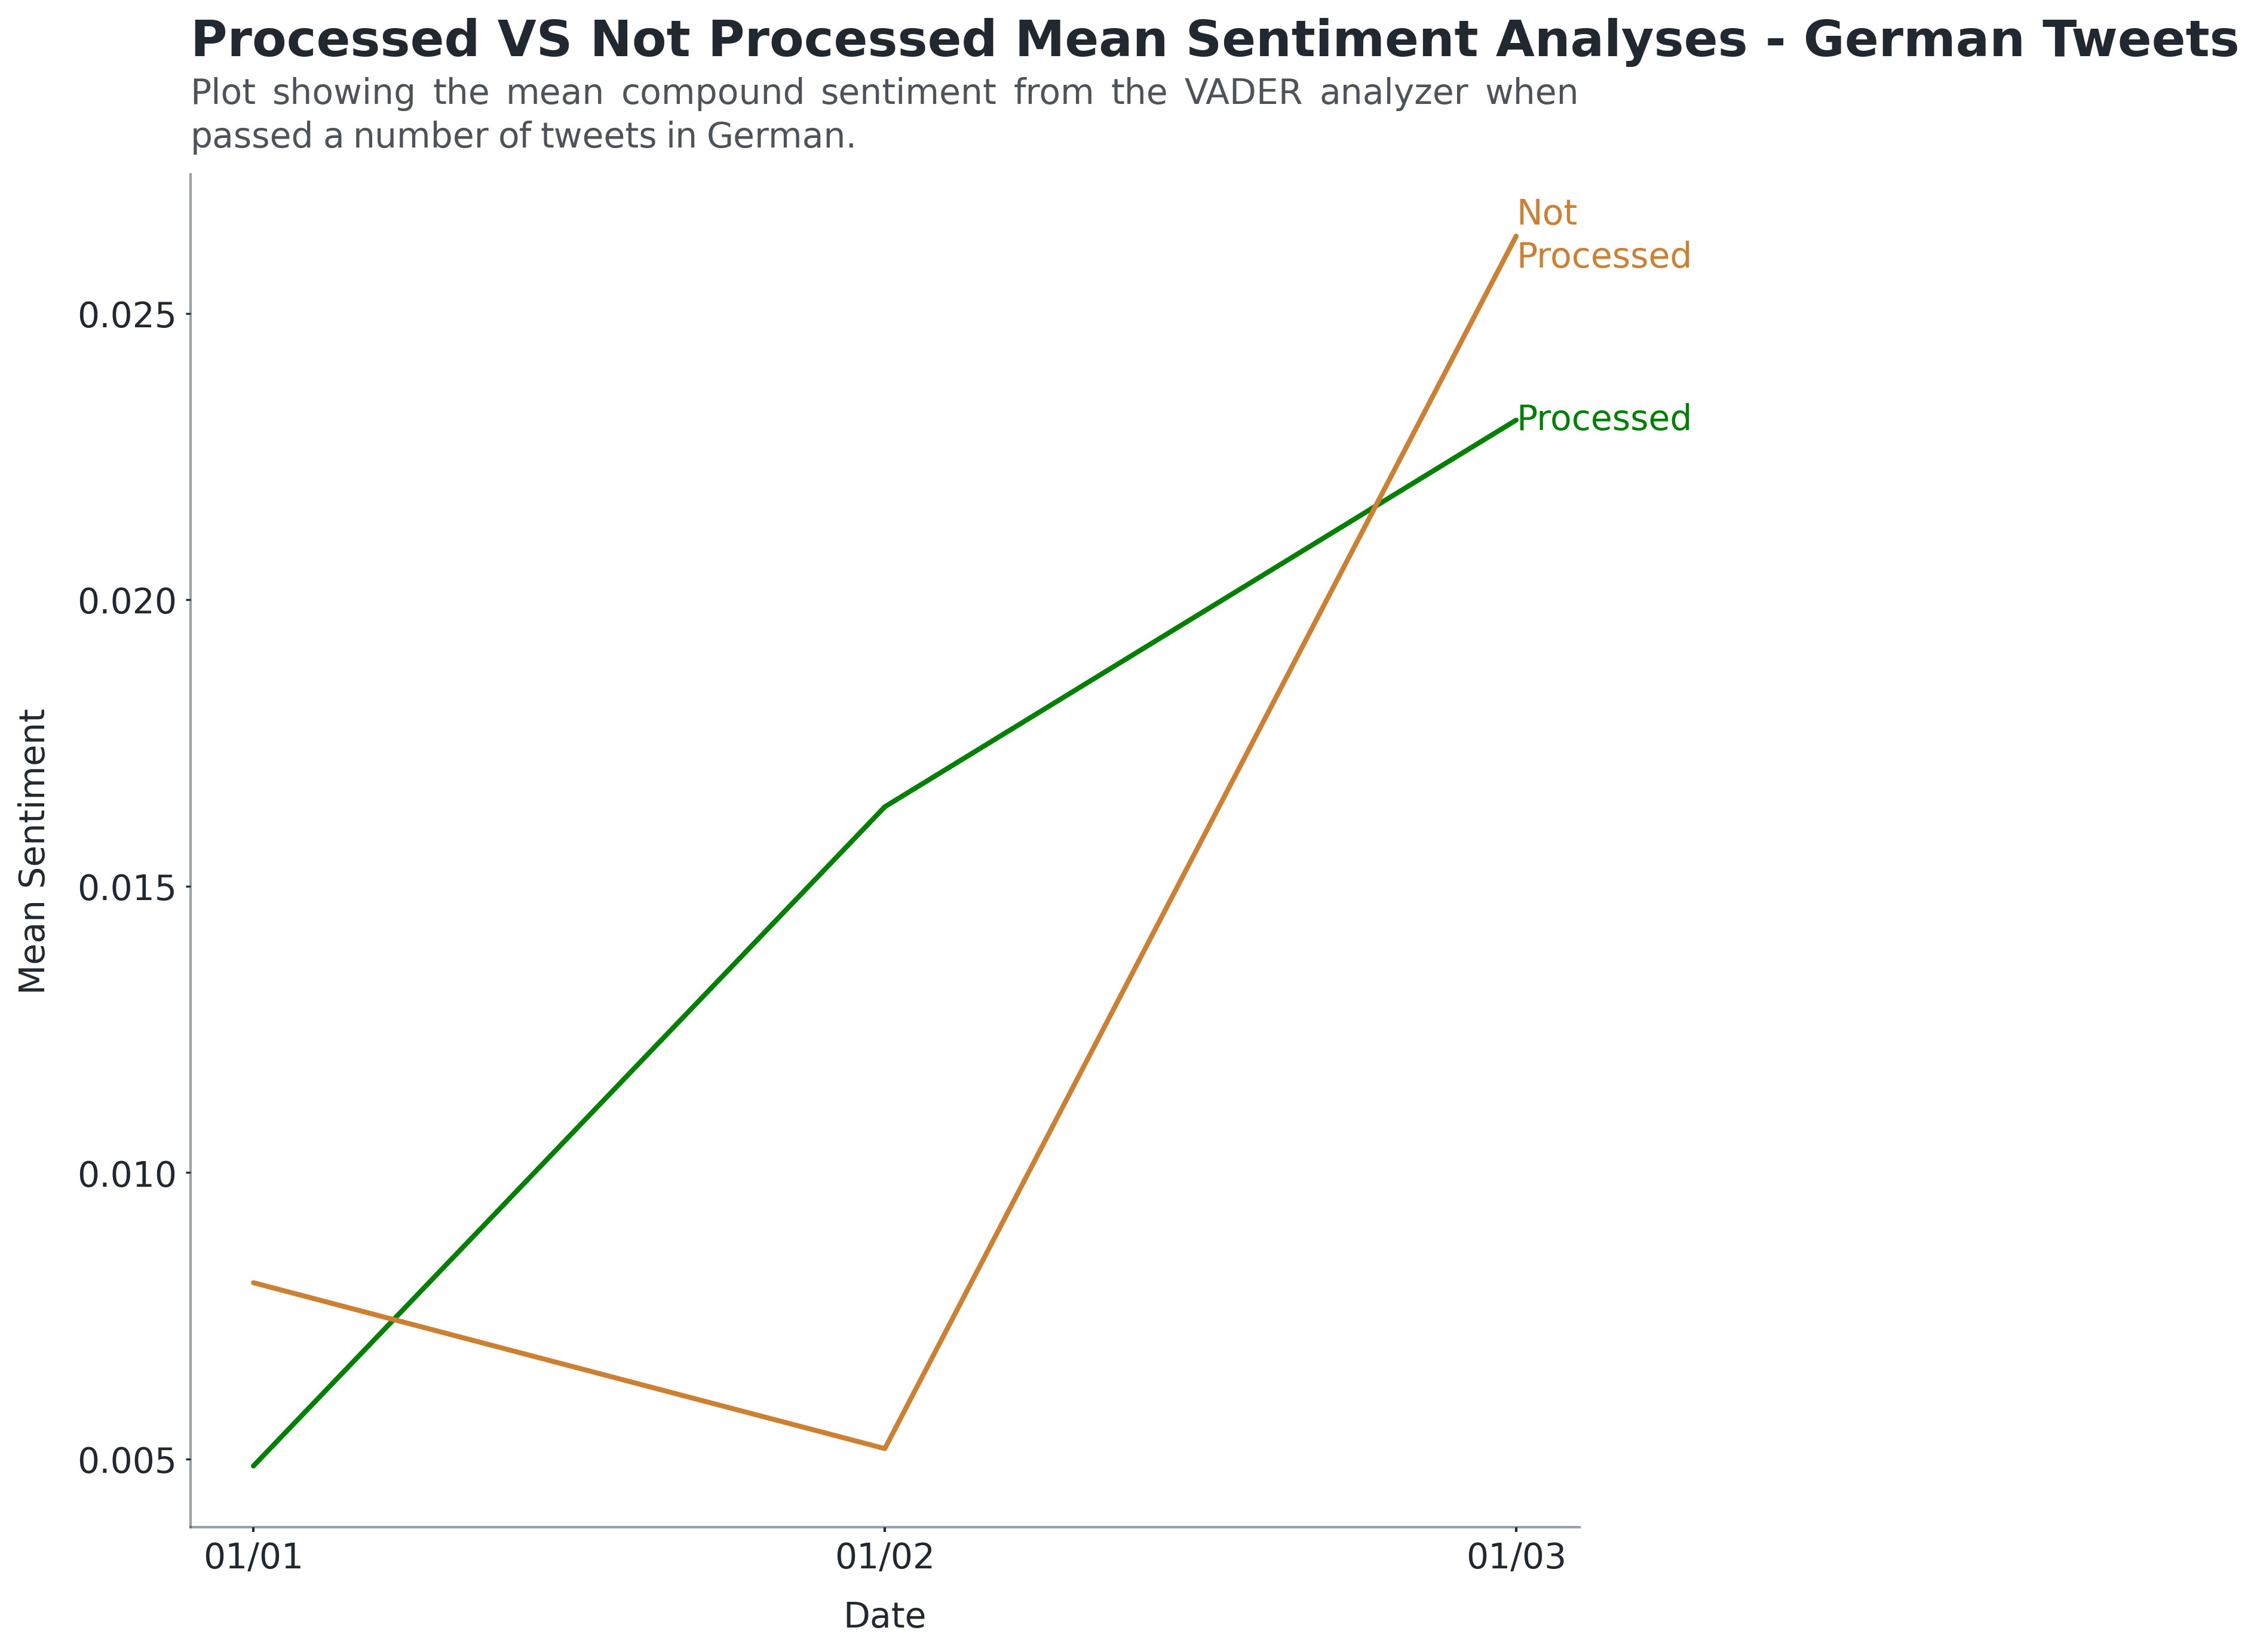
\includegraphics[width=\linewidth]{German Process VS NotProcessed.png}
  \caption{ }\label{fig:GermanPre}
\endminipage
\end{figure}

\noindent The difference calculated along with the shapes of the graphs plotted were not considered significant enough to remove pre-processing.
However the pre-process function was amended to keep more features like emojis and hashtags, which prior to this experiment where being removed.

\section{Daily Twitter Mean Sentiment}



\section{Daily Twitter Sentiment Classification}



\section{Daily Article vs Twitter Mean Sentiment}



\section{Daily Twitter Sentiment Classification with Article Mean Sentiment}



\section{Word Frequency in the Form of Word Clouds}

